% Copyright © 2013 Martin Ueding <dev@martin-ueding.de>
%
\input{header.tex}

\usepackage{tikz}

\newcommand{\themodul}{physik411}
\newcommand{\thegruppe}{Gruppe 2 -- Florian Seidler}
\newcommand{\theuebung}{3}

\ifoot{\footnotesize{Martin Ueding}}
\ihead{\themodul{} -- Übung \theuebung}
\ofoot{\footnotesize{\thegruppe}}

\def\thesubsection{\thesection\alph{subsection}}

\title{\themodul{} -- Übung \theuebung}
\subtitle{\thegruppe}
\author{
	Martin Ueding \footnote{\href{mailto:mu@uni-bonn.de}{mu@uni-bonn.de}}
}

\hypersetup{
	pdftitle={\themodul {} - Übung \theuebung},
}

\begin{document}

\maketitle

\begin{center}
	\ccbysadetitle
\end{center}

\begin{table}[h]
	\centering
	\begin{tabular}{l|c|c|c|c|c}
		Aufgabe
		& \ref 1
		& \ref 2
		& \ref 3
		& \ref 4
		& $\sum$   \\
		\hline
		Punkte
		& \punkte / 4
		& \punkte / 8
		& \punkte / 8
		& \punkte / 8
		& \punkte / 28
	\end{tabular}
\end{table}

%%%%%%%%%%%%%%%%%%%%%%%%%%%%%%%%%%%%%%%%%%%%%%%%%%%%%%%%%%%%%%%%%%%%%%%%%%%%%%%
%                                 Photoeffekt                                 %
%%%%%%%%%%%%%%%%%%%%%%%%%%%%%%%%%%%%%%%%%%%%%%%%%%%%%%%%%%%%%%%%%%%%%%%%%%%%%%%

\section{Photoeffekt}
\label 1

\subsection{Grenzwellenlänge}

\newcommand\UA{U_\text{A}}

Es muss $\hbar \omega \geq \UA$ gelten. Nach $f$ umgeformt bleibt:
\[
	f \geq \frac\UA h = \SI{5.08e14}\hertz
\]

Und die dazugehörige Wellenlänge:
\[
	\lambda \leq \frac{ch}\UA = \SI{5.90e-7}\meter
\]

\subsection{Geschwindigkeit}

Ich forme nach $v$ um:
\[
	h \frac c\lambda - \UA = \half m_\text{e} v^2
	\implies
	v = \SI{712000}{\meter\per\second}
\]

%%%%%%%%%%%%%%%%%%%%%%%%%%%%%%%%%%%%%%%%%%%%%%%%%%%%%%%%%%%%%%%%%%%%%%%%%%%%%%%
%             Energie-Impuls-Beziehungen und Comptonwellenlänge              %
%%%%%%%%%%%%%%%%%%%%%%%%%%%%%%%%%%%%%%%%%%%%%%%%%%%%%%%%%%%%%%%%%%%%%%%%%%%%%%%

\section{Energie-Impuls-Beziehungen und Comptonwellenlänge}
\label 2

\subsection{Diagramm}

Die kinetische Energie für ein klassisches Teilchen ist $E_\text{kin} =
p^2/(2m)$. Für ein relativistisches Teilchen mit Ruhemasse $E_0$ ist die
Gesamtenergie $E$: $E^2 = E_0^2 + c^2 p^2$. Dabei ist die kinetische Energie:
\[
	E_\text{kin} = \sqrt{E_0^2 + c^2 p^2} - E_0
\]

Für ein Photon ist $E_0 = 0$. In Abbildung \ref{fig:2-tikz} sind die
verschiedenen Formeln mit frei gewählten Parametern geplottet. In Abbildung
\ref{fig:2-mathematica} das ganze mit den richtigen Zahlenwerten, allerdings
weniger übersichtlich.

\begin{figure}
	\centering
	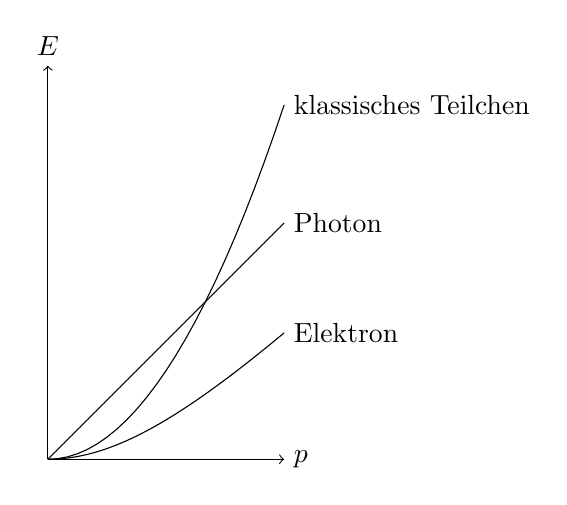
\begin{tikzpicture}[scale=2]
		\draw[->] (0, 0) -- ++(1.5, 0) node[right] {$p$};
		\draw[->] (0, 0) -- ++(0, 2.5) node[above] {$E$};
		\draw[domain=0:1.5] plot (\x, {\x}) node[right] {Photon};
		\draw[domain=0:1.5] plot (\x, {sqrt(1+\x^2) - 1}) node[right] {Elektron};
		\draw[domain=0:1.5] plot (\x, {\x^2}) node[right] {klassisches Teilchen};
	\end{tikzpicture}
	\caption{%
		Plot für die verschiedenen Teilchen. Für diesen Plot habe ich $c = h =
		1$ sowie für das Elektron $E_0 = m = 1$ gesetzt.
	}
	\label{fig:2-tikz}
\end{figure}

\begin{figure}
	\centering
	\includegraphics[width=.85\textwidth]{H2-Plot.pdf}
	\caption{%
		Plot der Energien für verschiedene Teilchen. In blau ist das klassische
		Elektron, in violett das Photon und in gelb das Elektron. In grün die
		Energie des Photons zur Compton-Wellenlänge. Auf der Ordinate ist der
		Impuls $p$ in $\si{\mega\electronvolt}/c$, auf der Abszisse die
		kinetische Energie $E$ in $\si\joule$.
	}
	\label{fig:2-mathematica}
\end{figure}

Für kleine Impulse sind die relativistische und die klassische Formel sehr nah
beieinander, wie zu erwarten ist.

\subsection{Compton-Wellenlänge}

Die Wellenzahl $k$ zur Compton-Wellenlänge ist:
\[
	k_\text{C} = \frac{2\piup}{\lambda_\text{C}} = \SI{2.84e12}{\radian\per\meter}
\]

Der Impuls dazu ist:
\[
	p_\text{C} = \hbar k_\text{C} = \SI{3.00e-22}{\kilogram\meter\per\second}
\]

Und die Energie:
\[
	E_\text{C} = cp_\text{C} = \SI{2.99e-22}\joule = \SI{.561}{\mega\electronvolt}
\]

Den Wert für $p_\text{C}$ habe ich nicht in Abbildung \ref{fig:2-mathematica}
eingezeichnet, da ich nicht weiß, wie in Mathematica eine vertikale Linie
eingefügt wird. Sie sollte aber bei \num{.56} liegen.

%%%%%%%%%%%%%%%%%%%%%%%%%%%%%%%%%%%%%%%%%%%%%%%%%%%%%%%%%%%%%%%%%%%%%%%%%%%%%%%
%            Atomares Magnetfeld, Kernmoment und Hyperfeinstruktur            %
%%%%%%%%%%%%%%%%%%%%%%%%%%%%%%%%%%%%%%%%%%%%%%%%%%%%%%%%%%%%%%%%%%%%%%%%%%%%%%%

\section{Atomares Magnetfeld, Kernmoment und Hyperfeinstruktur}
\label 3

\fehlt

%%%%%%%%%%%%%%%%%%%%%%%%%%%%%%%%%%%%%%%%%%%%%%%%%%%%%%%%%%%%%%%%%%%%%%%%%%%%%%%
%                            Stern-Gerlach-Versuch                            %
%%%%%%%%%%%%%%%%%%%%%%%%%%%%%%%%%%%%%%%%%%%%%%%%%%%%%%%%%%%%%%%%%%%%%%%%%%%%%%%

\section{Stern-Gerlach-Versuch}
\label 4

\fehlt

%%%%%%%%%%%%%%%%%%%%%%%%%%%%%%%%%%%%%%%%%%%%%%%%%%%%%%%%%%%%%%%%%%%%%%%%%%%%%%%
%                                    Ende                                     %
%%%%%%%%%%%%%%%%%%%%%%%%%%%%%%%%%%%%%%%%%%%%%%%%%%%%%%%%%%%%%%%%%%%%%%%%%%%%%%%

\IfFileExists{\bibliographyfile}{
	%\bibliography{\bibliographyfile}
}{}

\end{document}

% vim: spell spelllang=de
